\documentclass{math}

\usepackage{tikz}

\title{University Physics 1A}
\author{Alvin Lin}
\date{November 6th, 2017}

\begin{document}

\maketitle

\section*{Moment of Inertia}
Calculate \( I_{cm} \) for a flat, circular disk of mass \( M \) and radius
\( R \) with a uniform mass distribution. Choose the axis to be perpendicular to
the plane of the penny and passing through its center.
\begin{align*}
  \diff{A} &= 2\pi r\diff{r} \\
  \diff{m} &= \sigma\diff{A} = \sigma2\pi r\diff{r} \\
  &= \frac{M}{\pi r^2}2\pi r\diff{r} \\
  I &= \int r^2\diff{m} \\
  &= \int_{0}^{R}r^2\frac{M}{\pi R^2}2\pi r\diff{r} \\
  &= \frac{1}{2}MR^2
\end{align*}
Determine the moment of inertia of a thin triangular slab as show. Be careful
with the limits of integration. It has mass \( M \) uniformly distributed, and
dimensions as shown. There are still a couple of ways to make the slices, but
the answer should be the same way either way.
\begin{center}
  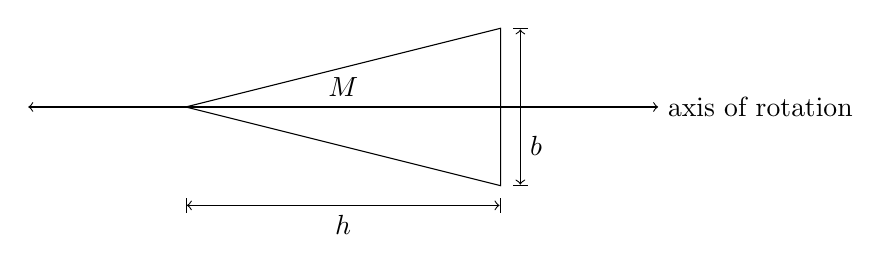
\begin{tikzpicture}
    \draw (0,0) -- (4,-1) -- (4,1) -- cycle
      node[pos=0.5,yshift=-0.25cm] {\( M \)};
    \draw[|<->|] (4.25,-1) -- (4.25,1) node[pos=0.25,right] {\( b \)};
    \draw[|<->|] (0,-1.25) -- (4,-1.25) node[pos=0.5,below] {\( h \)};
    \draw[<->] (-2,0) -- (6,0) node[right] {axis of rotation};
  \end{tikzpicture}
\end{center}
\begin{align*}
  y &= \frac{b}{2h}x \\
  \diff{A} &= (h-x)\diff{y} \\
  &= (h-\frac{2h}{b}y)\diff{y} \\
  \diff{m} &= \sigma\diff{A} \\
  &= \frac{M}{\frac{1}{2}bh}(h-\frac{2h}{b}y)\diff{y} \\
  I &= \int r^2\diff{m} \\
  &= 2\int r^2\diff{m} \\
  &= 2\int_{0}^{\frac{h}{2}}
    y^2\frac{M}{\frac{1}{2}bh}(h-\frac{2h}{b}y)\diff{y} \\
  &= \frac{1}{b}Mb^2
\end{align*}

\subsection*{Analogies between Linear and Rotational Motion}
\[ KE = \frac{1}{2}mv^2 = \frac{1}{2}m(r\omega)^2 \]
\[ KE = \frac{1}{2}I\omega^2 \]
Moment of inertia is analogous to mass.
\[ F_{net} = ma \]
\[ F_{net} = I\alpha \]

\begin{center}
  You can find all my notes at \url{http://omgimanerd.tech/notes}. If you have
  any questions, comments, or concerns, please contact me at
  alvin@omgimanerd.tech
\end{center}

\end{document}
